%! TeX program = lualatex
\documentclass[12pt,a4paper]{article}

\usepackage[nil]{babel}
\usepackage{unicode-math}
\usepackage[svgnames]{xcolor}
\usepackage{lmodern}
\usepackage{graphicx}
\usepackage{wrapfig}
\usepackage{float}
\usepackage{parskip}

\babelprovide[import=el, main, onchar=ids fonts]{greek} % can also do import=el-polyton
\babelprovide[import, onchar=ids fonts]{english}

\babelfont{rm}
          [Language=Default]{Liberation Sans}
\babelfont[english]{rm}
          [Language=Default]{Liberation Sans}
\babelfont{sf}
          [Language=Default]{Liberation Sans}
\babelfont{tt}
          [Language=Default]{Liberation Sans}

%Enter Title Here
 \title{Domain-model-v0.1 \\ LibShare}
\author{\textbf{Ονόματα / ΑΜ / Έτος:} \\ Γρηγόρης Καπαδούκας / 1072484 / 4\textdegree \\ Χρήστος Μπεστητζάνος / 1072615 / 4\textdegree \\ Νικόλαος Αυγέρης / 1067508 / 5\textdegree \\ Περικλής Κοροντζής / 1072563 / 4\textdegree}

\begin{document}

\makeatletter
\begin{center}
	\LARGE{\@title} \\
	\pagebreak
    \begin{LARGE}\@author\end{LARGE} 
    \pagebreak
\end{center}

%Insert Body Here
\section{Σχήμα Domain Model}

Στο Σχήμα \ref{Σχήμα Domain Model} φαίνεται το Domain Model για την εφαρμογή μας:

\begin{figure}[H]
	\makebox[\textwidth]{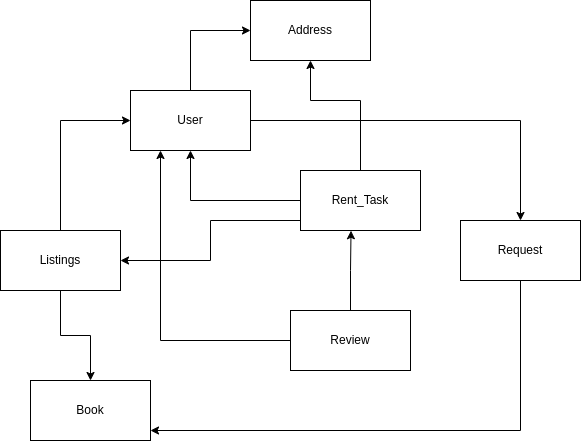
\includegraphics[width=\textwidth]{Domain model.png}}
	\caption{Σχήμα Domain Model}
	\label{Σχήμα Domain Model}
\end{figure}

\section{Σύντομη περιγραφή κλάσεων}

\subsection{User}
Ο κάθε χρήστης, θα περιέχει βασικές πληροφορίες όπως όνομα, ηλικία, ποσό στον λογαριασμό του κλπ.

\subsection{Book}
Τα βιβλία που έχουν εισαχθεί στο σύστημα (είτε είναι διαθέσιμα είτε όχι). Περιέχονται βασικές πληροφορίες των βιβλίων όπως τίτλος, συγγραφέας, είδος (πχ φαντασίας), κατηγορία (πχ νουβέλα).

\subsection{Rent Task}
Αποτελεί καταγραφή ενοικίασης ενός βιβλίου. Περιέχει δεδομένα όπως τον ιδιοκτήτη του βιβλίου (τύπου user), τον ενοικιαστή (τύπου user) το βιβλίο (τύπου Listing) την κατάσταση (σε τι κατάσταση βρίσκεται η διαδικασία, π.χ. "Ολοκληρωμένη", "Αναμένεται αποστολή" κ.α) και Tracking Number στη περίπτωση που γίνεται ταχυδρομική συναλλαγή.

\subsection{Review}
Μετά την ολοκλήρωση κάθε "Rent Task" οι χρήστες μπορούν να εισάγουν κριτική στους χρήστες με τους οποίους έκαναν την συναλλαγή (ιδιοκτήτη ή ενοικιαστή), μαζί με προαιρετικά σχόλια. Αυτές οι κριτικές αποτελούν στιγμιότυπα κλάσης Review και συνδέονται με το "Rent Task" που αφορούν, τον χρήστη που τις σύνταξε και τον χρήστη που αφορούν.

\subsection{Request}
Σε αυτό τον πίνακα αποθηκεύονται οι αιτήσεις που κάνουν οι χρήστες. Περιέχονται δεδομένα όπως: ο χρήστης που έκανε το request (τύπου User), το βιβλίο που ψάχνει (τύπου Book), την κατάσταση της αίτησης ("Ολοκληρωμένη" ή "Ενεργή") κ.α.

\subsection{Address}
Διευθύνσεις χρηστών που έχουν αποθηκευτεί στο σύστημα. Συνδέονται με το προφίλ κάθε χρήστη καθώς και με το "Rent Task" στο οποίο έγινε αποστολή κάποιου βιβλίου στην διεύθυνση αυτή.

\subsection{Listing}
Περιέχει τα βιβλία που προσφέρει ο χρήστης προς ενοικίαση. Έχει δεδομένα όπως: Ιδιοκτήτης βιβλίου (τύπου User), Βιβλίο (τύπου Book), τιμή κ.α.

\subsection{Favorites}
Περιέχει τους χρήστες τους οποίους ένας χρήστης “ακολουθεί” (δηλαδή έχει προσθέσει στην λίστα αγαπημένων του). Αποθηκεύεται ο χρήστης "αγαπημένος" και ο χρήστης που πρόσθεσε τον άλλον στη λίστα του.

\section{Συμμετοχή και Ρόλοι στη Συγγραφή του Κειμένου}
\begin{enumerate}
	\item \textbf{Περικλής Κοροντζής:} Author
	\item \textbf{Γρηγόρης Καπαδούκας:} Peer Reviewer
\end{enumerate}

\end{document}
